\section{Illustration}
\label{sec:app}

% when talking about BCN mention
% https://www.researchgate.net/publication/254457523_Urban_form_and_compactness_of_morphological_homogeneous_districts_in_Barcelona_towards_an_automatic_classification_of_similar_built-up_structures_in_the_city#

% all technical details in to an appendix tables from excel should go to notebooks

% spatial signature is a conceptual framework which can materialise in different ways
The classification of form and function into spatial signatures is a conceptual framework and
as such, can materialise in different ways depending on the particular implementation of
a description of both form and function and the method of aggregation of enclosed cells
into singatures.
% here we present it applied to five cases from around the world
In this section, we present an illustration of the concept applied to five
case studies reflecting different environments and heterogeneous input data.
We choose this diversity to demonstrate the ability to adapt the
classification to rather different situations.
% the sample comes with geographical variation - 1, 2, 3, 4, 5
The five cities are displayed in Figure \ref{fig:world_map}.
The sample offers geographical variation covering Europe (Barcelona, Spain), North
America (Houston, TX, United States), South America (Medellin, Colombia), Africa (Dar es
Salaam, Tanzania) and South-east Asia (Singapore),
% that brings different culture, development, planning paradigm, historical and social
% contexts
coupled with cultural diversity, different planning paradigms involved in shaping the
respective environments as well as varied historical and social contexts in which the
selected cities were built and developed.
% at the same time, it brings different input data, varied in both quality and richness
At the same time, the selection brings a variety of input data covering both extremes in
terms of quality (e.g., official mapping in Barcelona vs remote sensing in Houston), the
richness of information on functional aspects of places (e.g., detailed data on the
municipal level in Medellin vs global gridded datasets in Dar es Salaam) and scale
(82,375 units in Barcelona vs 2,043,581 units in Houston).
% we present this variety to illustrate the application and flexibility of the concept
We present this variety to illustrate the flexibility of spatial signatures to
accommodate varied inputs and adapt to a local specificity, while retaining the merit of
the concept.

\begin{figure}
    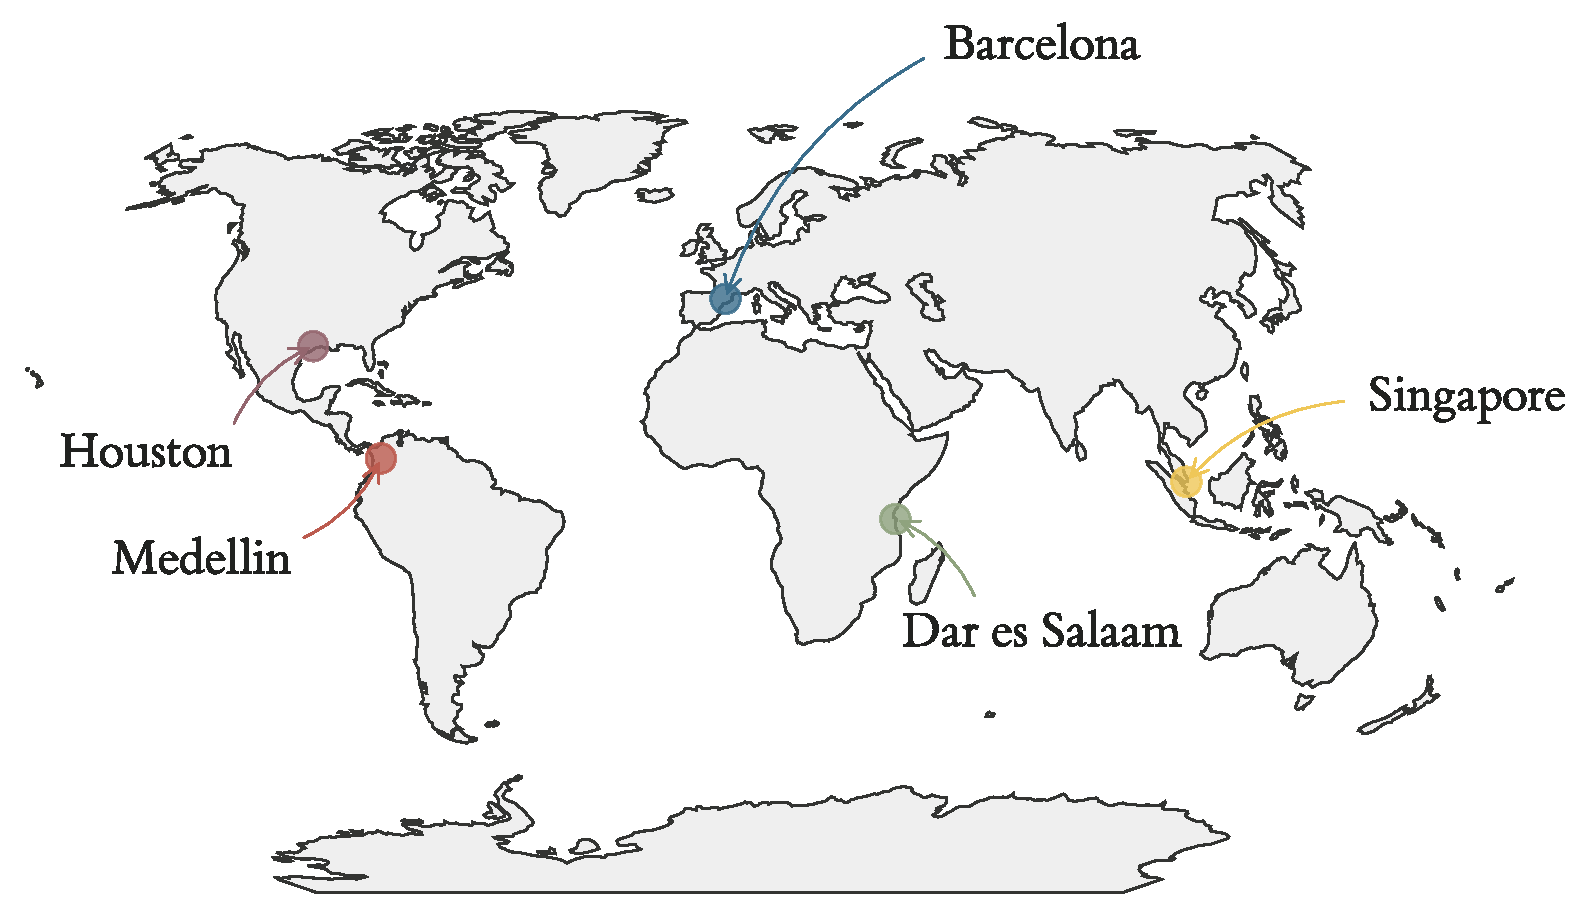
\includegraphics[width=0.75\linewidth, center]{figures/examples_map.pdf}
    \caption{Selection of case studies covering geographical variation,
    cultural diversity, different planning paradigms involved in shaping the
    respective environments as well as varied historical and social contexts in which the
    selected cities were built.}
    \label{fig:world_map}
\end{figure}

\subsection{Method}
%%%%%%%%%%%% Structure 4.1 (squeeze it in a page) introduction of cases - 1 per
% continent; geographical variation, take different cities, cultures, historical moments

%% method - top level outline of the method. Data, Form + convolution, Function,
% Clustering One para on how to build the data - F+F+Convolution, how it varies across
% examples (link to App.)

%%% shall we add conceptual diagram of the method?

% 1. data retrieval from open sources
The delineation of spatial signatures starts with the input data reflecting form and
function of each place. We use enclosed tessellation, outlined in Section
\ref{ssec:ss_et}, as the core spatial unit. Therefore, the input
data consists of building footprints and physical barriers --delimiters-- denoting streets,
railways, and water bodies.
% 2. geographies - enclosures, enclosed tessellation
Using these delimiters, we first identify the geometry of enclosures, which we
combine with building footprints to grow ET cells.
% 3. characterization of form - primary + convolutions
The resulting set allows for a comprehensive morphometric analysis
composed of characters capturing individual aspects of form, and
contextualisation, following the model proposed by
\citealp{fleischmann2021methodological}. In the latter, we
include the distribution of each character within the neighbouring context of each
tessellation cell.
% 4. characterisation of function
Function is captured as a heterogeneous set of characteristics reflecting
features from
population density to location of amenities. All aspects are linked to ET cells
using the most appropriate method for each data input (e.g., areal
        interpolation,
network accessibility). The complete list of used characters relfecting both form and
function, as well as implementation details are available in \ref{sec:appendix}.

% Second para on how we generate signatures (clustering); once we have those we
% dissolve.

% 5. cluster analysis input (all linked to cell)
Spatial signatures are then identified using cluster analysis on the
form-function characteristics attached to ET cells. 
% 6. clustergram
The combined data reflecting both form and function are therefore standardised and
clustered using K-Means. Since the number of classes is not known a priori,
we use clustergrams \citep{schonlau2002clustergram} to understand the
behaviour of different solutions and select the optimal number of groups.
\ref{sec:appendix} contains details on the clustergrams used.
% 7. clustering
The final clustering is run with 1000 initialisations to ensure stability of
results.
% 8. dissolution
Once clustered, we
dissolve the boundaries of contiguous ET cells assigned into the same cluster to
create instances of spatial signatures.


\subsection{Results}
% 4.2 (a page and a half) Results; tell some stories to get reader on board

%%% Para1 how to read the map in an applied way geometries reflect boundaries of spatial
% signatures
Figures \ref{fig:maps1}-\ref{fig:maps2} illustrate the resulting spatial signatures in the respective case
studies. The geometries reflect the spatial extent of individual signatures
derived from the enclosed tessellation
% colours reflect a type of a signature - two areas within the same type share the
% characteristics; similarity of colours has no meaning
with colour coding reflecting the type of a signature, i.e. the initial cluster. Two
areas within the same type are expected to share form and function characteristics, being more similar to each other than to the
other classes. Note that the similarity of different colours does not encode
similarity of signatures.

\begin{figure}
    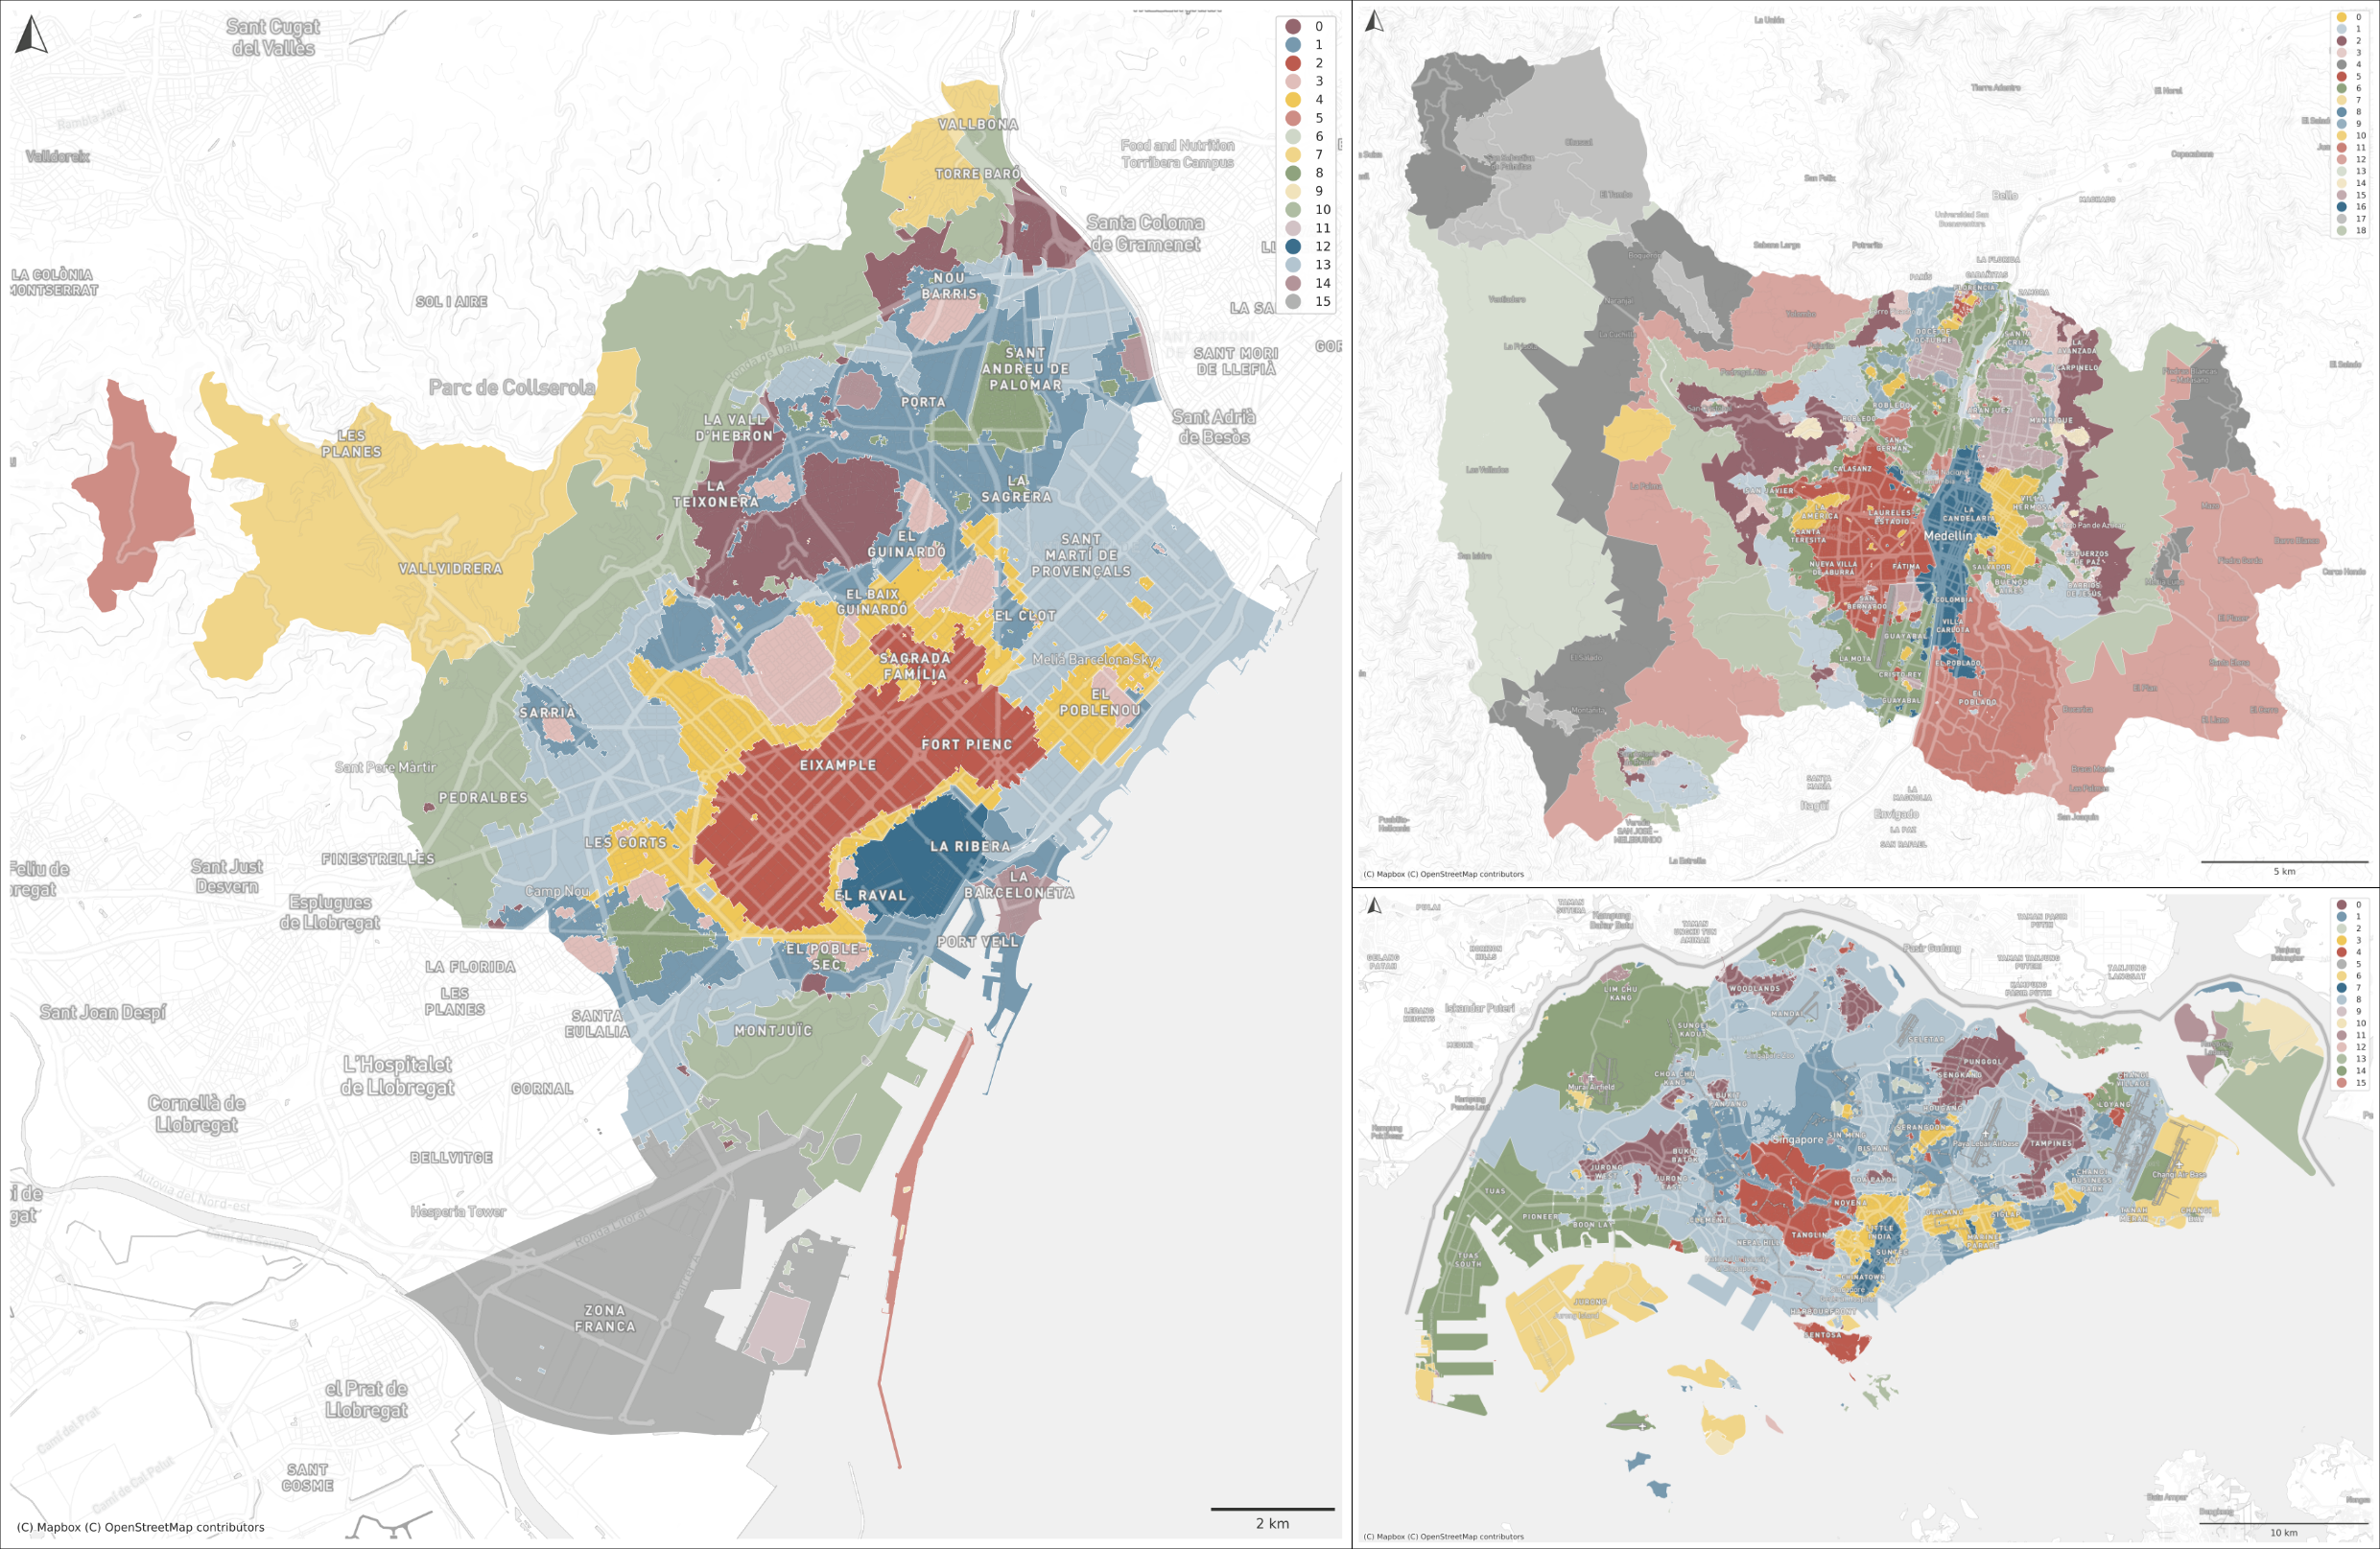
\includegraphics[width=\linewidth]{figures/maps1.png}
    \caption{Resulting Spatial Signatures in the case of Barcelona (A), Singapore (B)
    and Medellin (C). Colours are used to distinguish between types within a
    single case. Note scale differs across maps given the different extent
    covered by each urban area.}
    \label{fig:maps1}
\end{figure}

%%% Para2 things which are shared/consistent 9-19 clusters, not dependent on the scale
% but reflecting the heterogeneity of a place
The granularity of classification, that is the number of clases identified
through the clustergram, ranges from nine (Houston) to 19 (Medellin) signature
types. However, it is interesting the actual number is not dependent on the size of each
city but rather on the heterogeneity in form and function of each place. This
phenomenon is best illustrated on the comparison
between Houston and Barcelona, the largest (2 million cells) and the smallest (80 thousand
cells) case. Houston, archetype of North American, post WW-II sprawling urban fabric shows
considerably smaller diversity of spatial patterns (nine spatial signature
types) than
Barcelona (16 types).
% core clusters and outlier clusters - the abundance varies a lot
The distribution of cluster sizes follows the same unequal pattern across
all cases. The most extensive types contain between 15\% and 28\% of all
observations, gradually decreasing towards a small number of
outlier clusters containing less than one per cent of all observations within each sample.
% transition from core to countryside - singapore is exception, its island nature
% restricts such behaviour
All illustrations include both extremes on the urbanisation continuum, with delineated
central districts on the one hand and non-urban countryside signatures on the
other. We interpret this
transition as a gradual move from more urban signatures to less so. The only
exception where this pattern is not as clear (but
still present) is Singapore, whose geographical extent is limited to the
the main island and thus does not allow for full transition.

%%% Para3 interesting stories from cases (BCN village centres, DeS slums) BCN reflects
% its historical origin - pre-industrial core and village centes, later filled by
% eixample, which has its homogenous core and areas blending into the existing fabric
Barcelona is known for its extension grid (``Eixample''), which is captured as
a unique signature (red).
However, this development is historically an infill between the city's medieval core and
smaller preexisting peripheric settlements. Both core and periphery are
reflected in the typology of signatures, which embody these historical
origins. The spatial transition between historical organic fabric and the
heavily planned
Eixample is reflected as another signature (yellow), stitching together different patterns into a coherent city.
% Medellin's change of the pattern as we go up the hill from the central valley
% - central plateu allows more rigid planning reflected in several classes, hillsides
%   are becoming more vernacular
The spatial distribution of signatures in Medellin tells the story of its intricate
topography, even though the input data do not contain any explicit information
on it. The
city lies in a valley surrounded by steep slopes. While the central parts are
found on the
relatively flat terrain allowing paradigmatic planning and regularity of form
and function, hillsides become more vernacular leading to a sharp urban edge where
topography limits further development.

\begin{figure}
    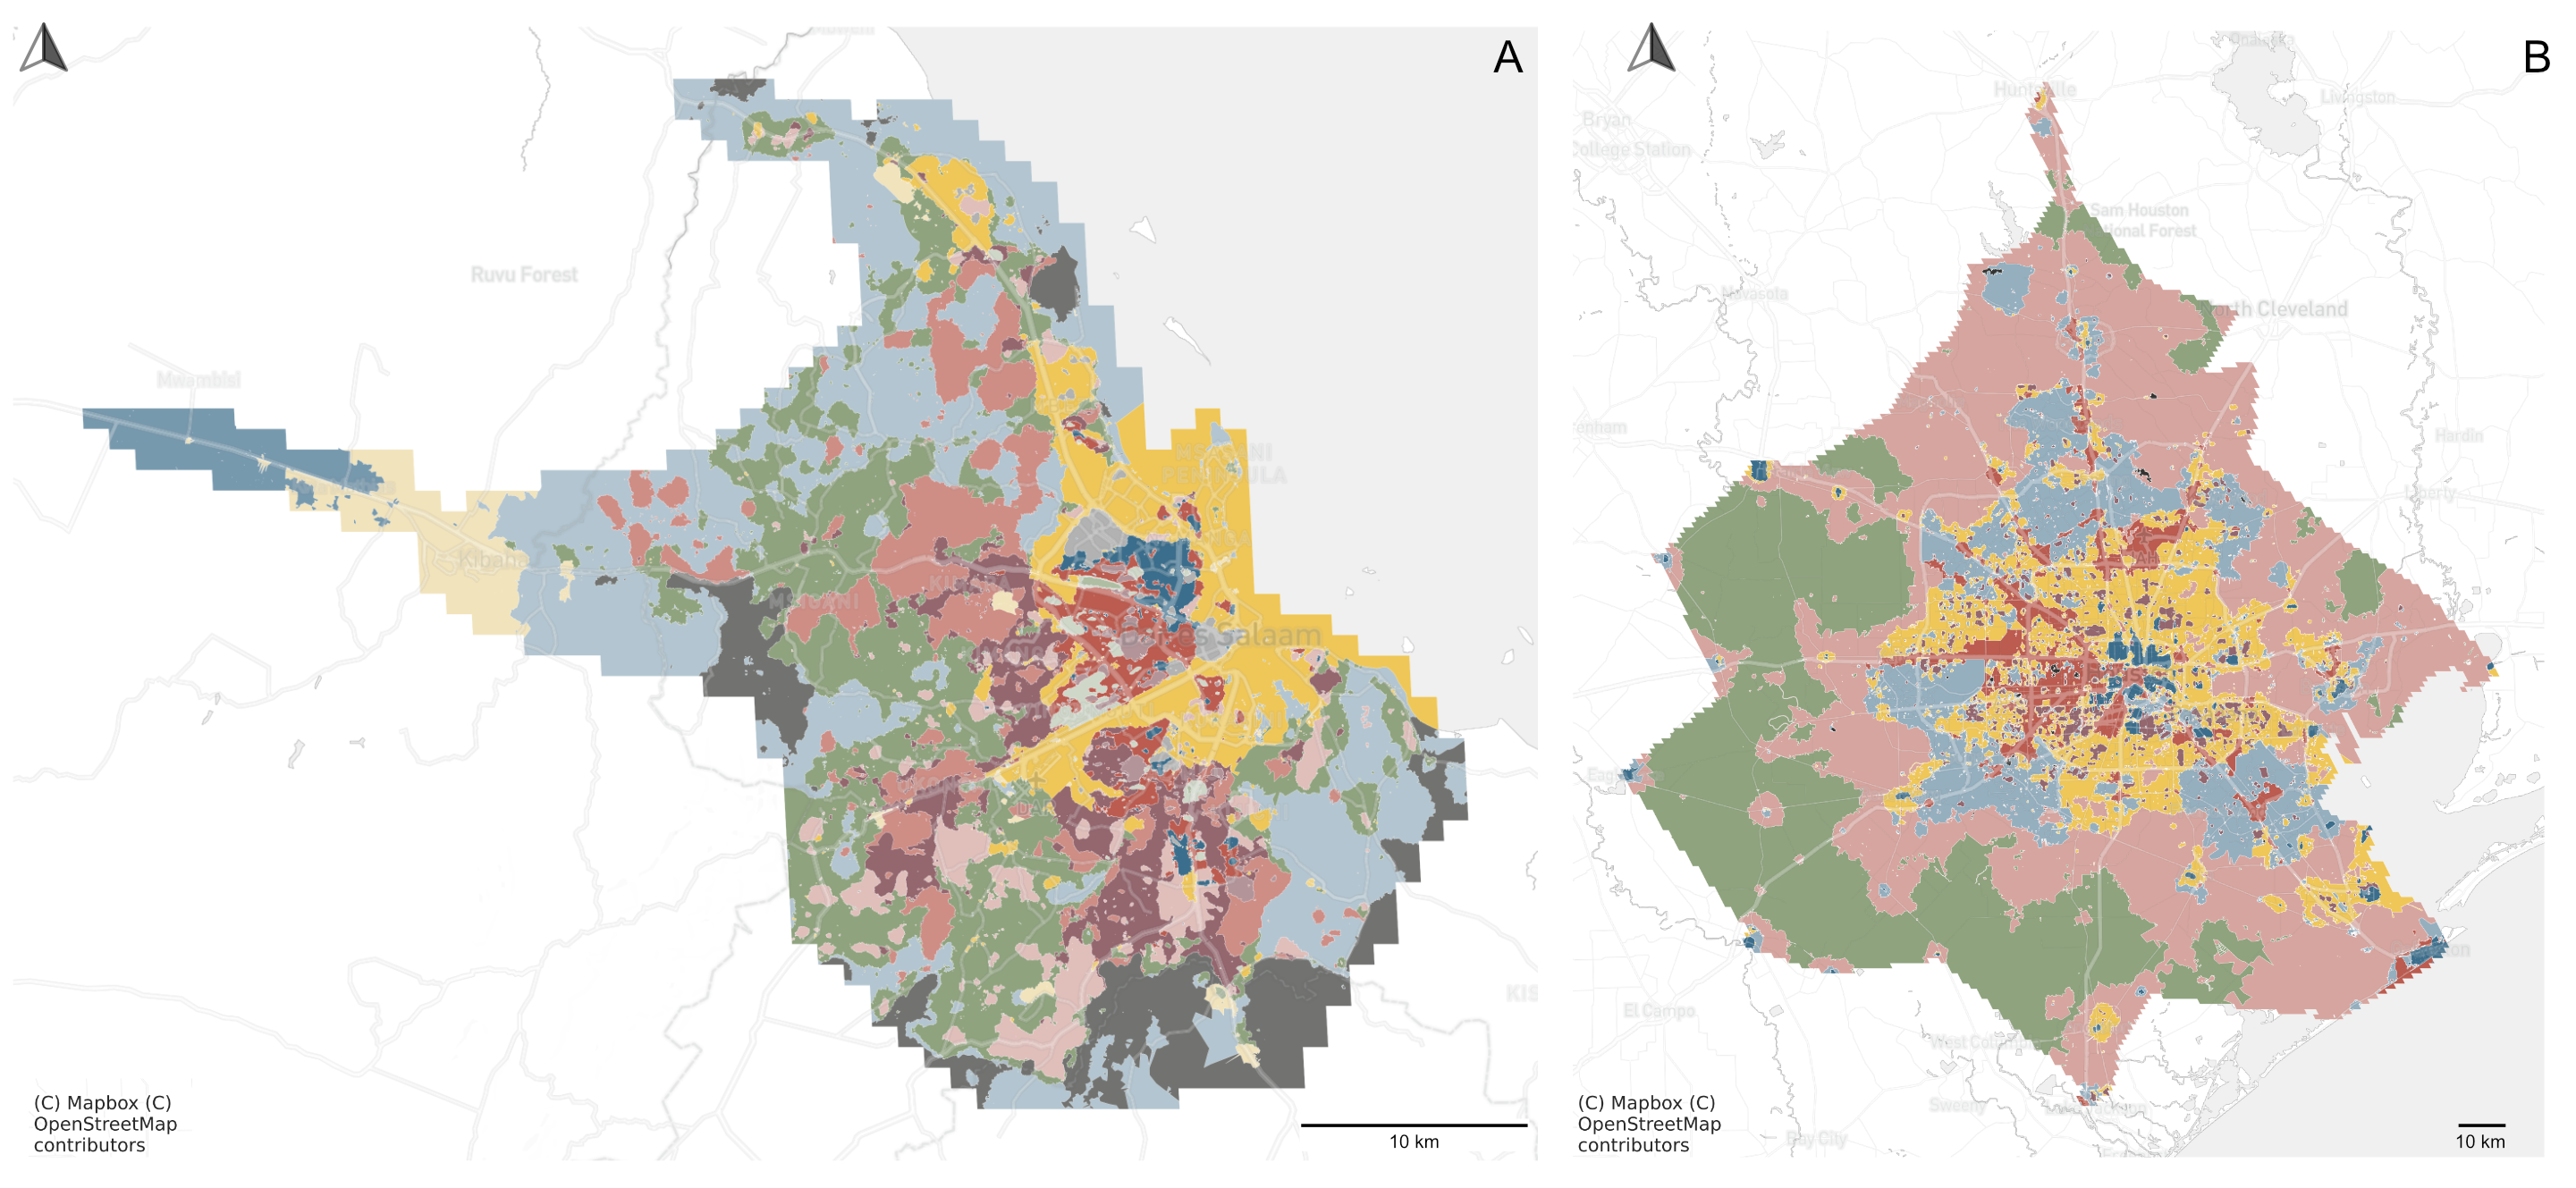
\includegraphics[width=\linewidth]{figures/maps2.png}
    \caption{Resulting Spatial Signatures in the case of Dar es Salaam (A) and Houston (B).
    Colours are used to distinguish between types within a single case.}
    \label{fig:maps2}
\end{figure}

% Dar es Salaam signatures capture different levels of formality, planned, semi-formal
% to informal
Signatures in Dar es Salaam reflect changes in the degree of formality in development, with
formal areas (yellow) distributed across the central parts of the city, in the vicinity
of the
coastline. The transition between different degrees of formality is not always gradual
as most informal parts of the city (light green and dark blue) appear as
infills of the space not occupied by more planned neighbourhoods.

% houston and its homogenous sprawl, changing its nature of sprawlness along the time
% and growth, with major roads forming spines of non-residential development
The character of spatial signatures in Houston follows two primary principles.
One  
forms the spine of activity spreading from the city centre radially to the suburbs. The
other fills the areas in-between the former, suggesting the decline of
compact, walkable urban blocks into the convoluted, dendritic street network patterns of
modern suburbs. The change in these predominantly residential signatures is gradual and
reflects the waves of development the city has experience during the post-war
period.
% NOTE: Houston signatures are not able to distinguish CBD from the rest of the "spine",
% shall we dicuss that at some point?

% Singapore singature tell the story of its growth. we can follow individual clusters
% and link their origin to different time periods
A similar situation can be found in Singapore, where different types of signatures can be linked
to the period when they were developed. Contrary
to previous cases, this evolution and, consequently, spatial signatures
followed a radial pattern. This process is not entirely contiguous, and thus
appear major infills built in the last 50 years.
